%this template was developed by Lasse D. Skaalum 
%but based on Jesper Kjær Nielsens template: https://github.com/jkjaer/aauLatexTemplates
\documentclass[11pt,oneside,a4paper]{report}
%%%%%%%%%%%%%%%%%%%%%%%%%%%%%%%%%%%%%%%%%%%%%%%%
% Language, Encoding and Fonts
% http://en.wikibooks.org/wiki/LaTeX/Internationalization
%%%%%%%%%%%%%%%%%%%%%%%%%%%%%%%%%%%%%%%%%%%%%%%%
% Select encoding of your inputs. Depends on
% your operating system and its default input
% encoding. Typically, you should use
%   Linux  : utf8 (most modern Linux distributions)
%            latin1 
%   Windows: ansinew
%            latin1 (works in most cases)
%   Mac    : applemac
% Notice that you can manually change the input
% encoding of your files by selecting "save as"
% an select the desired input encoding. 
\usepackage[utf8]{inputenc}
% Make latex understand and use the typographic
% rules of the language used in the document.
\usepackage{csquotes}
\usepackage[danish,english]{babel}
% Use the palatino font
\usepackage[sc]{mathpazo}
% Set space between lines
\usepackage{setspace}
% Choose the font encoding
\usepackage[T1]{fontenc}
% Remove page numbers from toc
\usepackage{tocloft}
% Itemize customization
\usepackage{enumitem}
\usepackage{multicol}
% Appendix environment
% \usepackage[title,titletoc]{appendix}

%%%%%%%%%%%%%%%%%%%%%%%%%%%%%%%%%%%%%%%%%%%%%%%%
% Graphics and Tables
% http://en.wikibooks.org/wiki/LaTeX/Importing_Graphics
% http://en.wikibooks.org/wiki/LaTeX/Tables
% http://en.wikibooks.org/wiki/LaTeX/Colors
%%%%%%%%%%%%%%%%%%%%%%%%%%%%%%%%%%%%%%%%%%%%%%%%
% load a colour package
\usepackage{xcolor}
\definecolor{aaublue}{RGB}{33,26,82}% dark blue
% The standard graphics inclusion package
\usepackage{graphicx}
% Set up how figure and table captions are displayed
\usepackage{caption}
\captionsetup{%
  font=footnotesize,% set font size to footnotesize
  labelfont=bf % bold label (e.g., Figure 3.2) font
}
% Adds \HUGE and \ssmall. The latter fills the gap between \scriptsize and \tiny.
\usepackage{moresize}
% Make the standard latex tables look so much better
% \usepackage{array,booktabs}
% ...or you can use this package instead
\usepackage{tcolorbox}
% Define a basic grey box with three custom params.
\newtcolorbox[auto counter,number within=section]{greybox}[3][]{
    title=#3~\thetcbcounter: #2,#1,title filled
}
% Enable the [H] option for figures and tables
\usepackage{float}
% Enable the use of frames around, e.g., theorems
\usepackage{framed}
% Adds support for full page background picture
\usepackage[contents={},color=gray]{background}
%\usepackage[contents=draft,color=gray]{background}

%%%%%%%%%%%%%%%%%%%%%%%%%%%%%%%%%%%%%%%%%%%%%%%%
% Mathematics
% http://en.wikibooks.org/wiki/LaTeX/Mathematics
%%%%%%%%%%%%%%%%%%%%%%%%%%%%%%%%%%%%%%%%%%%%%%%%
% Defines new environments such as equation,
% align and split 
\usepackage{amsmath}
% Adds new math symbols
\usepackage{amssymb}
% Use theorems in your document
% The ntheorem package is also used for the example environment
% When using thmmarks, amsmath must be an option as well. Otherwise \eqref doesn't work anymore.
\usepackage[framed,amsmath,thmmarks]{ntheorem}

%%%%%%%%%%%%%%%%%%%%%%%%%%%%%%%%%%%%%%%%%%%%%%%%
% Listings (Code Snippets)
% https://en.wikibooks.org/wiki/LaTeX/Source_Code_Listings
%%%%%%%%%%%%%%%%%%%%%%%%%%%%%%%%%%%%%%%%%%%%%%%%
\usepackage{listings}
\usepackage{color}

\renewcommand{\lstlistingname}{Code Snippet} % Listing -> Code Snippet
\definecolor{lighter-gray}{RGB}{240,240,240}

\lstset{
  backgroundcolor=\color{lighter-gray},
  extendedchars=true,
  basicstyle=\footnotesize\ttfamily,
  showstringspaces=false,
  showspaces=false,
  numbers=left,
  tabsize=4,
  breaklines=true,
  showtabs=false,
  captionpos=b,
  numberstyle=\footnotesize,
  numbersep=5pt
}

% Define C# as a snippet language.
\usepackage{courier}

\definecolor{Green}{rgb}{0, 0.3, 0}
\definecolor{DarkCyan}{rgb}{0, 0.545, 0.545}
\definecolor{Navy}{rgb}{0, 0, 0.5}
\definecolor{Teal}{rgb}{0, 0.5, 0.5}
\definecolor{DarkGray}{gray}{0.66}
\definecolor{Olive}{rgb}{0.5, 0.5, 0}
\definecolor{Pink}{rgb}{1.0, 0.75, 0.8}
\definecolor{DeepPink}{rgb}{1, 0.08, 0.58}
\definecolor{Brown}{rgb}{0.65, 0.165, 0.165}
\definecolor{DarkViolet}{rgb}{0.58, 0, 0.83}
\definecolor{SaddleBrown}{rgb}{0.55, 0.27, 0.07}
\lstdefinelanguage{CSharp}{
  morecomment = [l]{//}, 
  morecomment = [l]{///},
  morecomment = [s]{/*}{*/},
  morestring=[b]", 
  morestring=[b]',
  basicstyle=\footnotesize\ttfamily,
  commentstyle=\color{Green}\textit,
  stringstyle=\color{blue},
  sensitive = true,
  morekeywords=[1]{this, base},
  keywordstyle=[1]\bfseries,
  morekeywords=[2]{as, is, new, sizeof, typeof, true, false, stackalloc},
  keywordstyle=[2]\color{DarkCyan}\bfseries,
  morekeywords=[3]{else, if, switch, case, default,
  do, for, foreach, while, in},
  keywordstyle=[3]\color{blue}\bfseries ,
  morekeywords=[4]{break, continue, goto, return,
  yield, partial, global, where},
  keywordstyle=[4]\color{Navy},
  morekeywords=[5]{try, throw, catch, finally},
  keywordstyle=[5]\color{Teal}\bfseries,
  morekeywords=[6]{checked, unchecked},
  keywordstyle=[6]\color{DarkGray}\bfseries,
  morekeywords=[7]{fixed, unsafe},
  keywordstyle=[7]\color{Olive},
  morekeywords=[8]{bool, byte, sbyte, char, short, ushort, int, uint, long, ulong, float,
  double, decimal, enum, struct},
  keywordstyle=[8]\bfseries\color{red},
  morekeywords=[9]{class, interface, delegate, object, string,
  void},
  keywordstyle=[9]\color{red},
  morekeywords=[10]{explicit, implicit, operator},
  keywordstyle=[10]\color{Pink}\bfseries,
  morekeywords=[11]{params, ref, out},
  keywordstyle=[11]\bfseries\color{DeepPink},
  morekeywords=[12]{private, protected, internal, public},
  keywordstyle=[12]\bfseries\color{blue},
  morekeywords=[13]{abstract, const, event, var, override, virtual, volatile, extern, readonly, sealed, static},
  keywordstyle=[13]\color{Brown},
  morekeywords=[14]{namespace, using},
  keywordstyle=[14]\bfseries\color{Green},
  morekeywords=[15]{lock},
  keywordstyle=[15]\color{DarkViolet},
  morekeywords=[16]{get, set, add, remove},
  keywordstyle=[16]\color{SaddleBrown},
  morekeywords=[17]{null, value},
  keywordstyle=[17]\bfseries,
}

%%%%%%%%%%%%%%%%%%%%%%%%%%%%%%%%%%%%%%%%%%%%%%%%
% Page Layout
% http://en.wikibooks.org/wiki/LaTeX/Page_Layout
%%%%%%%%%%%%%%%%%%%%%%%%%%%%%%%%%%%%%%%%%%%%%%%%
% Change margins, papersize, etc of the document
\usepackage[
    top    = 3.50cm,
    bottom = 3.50cm,
    left   = 2.50cm,
    right  = 2.50cm
]{geometry}
% Modify how \chapter, \section, etc. look
% The titlesec package is very configureable
\usepackage{titlesec}
\titleformat{\chapter}{\normalfont\Huge\bfseries}{\thechapter}{20pt}{\Huge}
\titlespacing*{\chapter}{0pt}{3.5ex plus 1ex minus .2ex}{2.3ex plus .2ex}%less spacing above chapter title
\titleformat*{\section}{\normalfont\Large\bfseries}
\titleformat*{\subsection}{\normalfont\large\bfseries}
\titleformat*{\subsubsection}{\normalfont\normalsize\bfseries}
%\titleformat*{\paragraph}{\normalfont\normalsize\bfseries}
%\titleformat*{\subparagraph}{\normalfont\normalsize\bfseries}
%\setlength{\parindent}{0pt}%remove indentation on newline

% Change the headers and footers
\usepackage{fancyhdr}
\pagestyle{fancy}
\fancyhf{} %delete everything
\renewcommand{\headrulewidth}{0pt} %remove the horizontal line in the header
\setlength{\headheight}{14pt}
\renewcommand{\chaptermark}[1]{\markboth{\MakeUppercase{\ \thechapter.\ #1}}{}}%removes "Chapter" from \leftmark
% Define headers
\lhead{\small\nouppercase\leftmark} %left side of head
\rhead{\small\nouppercase\rightmark} %right side of head
% Define footers
\newcommand{\rightfoot}{\small Page \textbf{\thepage} of \textbf{\pageref{bib:mybiblio}}}
\newcommand{\leftfoot}{\small\authorname}
\rfoot{\rightfoot}%page number on all pages
\lfoot{\leftfoot}%group name on all pages
% Redefine the plain page style to modify footers on chapter pages
\fancypagestyle{plain}{%
    \fancyhf{} %delete everything
    \rfoot{\rightfoot} %page number on all chapter pages
    \lfoot{\leftfoot}%group name on all chapter pages
}

% Applies settings to appendix environment
\newcommand{\applyappendixconfig}{
    \addcontentsline{toc}{chapter}{Appendices}
    \renewcommand{\thesection}{\Alph{section}}
    % Hide page numbering in toc
    \addtocontents{toc}{\cftpagenumbersoff{chapter}}
    \addtocontents{toc}{\cftpagenumbersoff{section}}
    \addtocontents{toc}{\cftpagenumbersoff{subsection}}
    \addtocontents{toc}{\cftpagenumbersoff{subsubsection}}
    % Add appendices chapter without chapter number
    \chapter*{Appendices}
    \phantomsection
    % Remove head and foot from appendices
    \emptyheadfoot % Custom command to make head and foot empty
}

% Remove head and foot (Used in \applyappendixconfig)
\newcommand{\emptyheadfoot}{
    \rhead{ }
    \lhead{ }
    \rfoot{ }
    \lfoot{ }
    % Redefine the plain page style to modify footers on chapter pages
    \fancypagestyle{plain}{
        \fancyhf{} %delete everything
        \rfoot{ }
        \lfoot{ }
    }
}

% Do not stretch the content of a page. Instead,
% insert white space at the bottom of the page
\raggedbottom
% Enable arithmetics with length. Useful when
% typesetting the layout.
\usepackage{calc}

%%%%%%%%%%%%%%%%%%%%%%%%%%%%%%%%%%%%%%%%%%%%%%%%
% Bibliography
% http://en.wikibooks.org/wiki/LaTeX/Bibliography_Management
%%%%%%%%%%%%%%%%%%%%%%%%%%%%%%%%%%%%%%%%%%%%%%%%
\usepackage[backend=bibtex,
  bibencoding=utf8,
  style=ieee
  ]{biblatex}
\addbibresource{bib/bibliography}

%%%%%%%%%%%%%%%%%%%%%%%%%%%%%%%%%%%%%%%%%%%%%%%%
% Misc
%%%%%%%%%%%%%%%%%%%%%%%%%%%%%%%%%%%%%%%%%%%%%%%%
% Add bibliography and index to the table of contents
\usepackage[nottoc]{tocbibind}
% Used to place fixme/todo notes as notes in the footer
% Full documentation: https://www.lrde.epita.fr/~didier/software/fixme.pdf
\usepackage[footnote,english,draft,silent,nomargin]{fixme}
% Mock text
\usepackage{lipsum}

%%%%%%%%%%%%%%%%%%%%%%%%%%%%%%%%%%%%%%%%%%%%%%%%
% Hyperlinks
% http://en.wikibooks.org/wiki/LaTeX/Hyperlinks
%%%%%%%%%%%%%%%%%%%%%%%%%%%%%%%%%%%%%%%%%%%%%%%%
% Enable hyperlinks and insert info into the pdf
% file. Hypperref should be loaded as one of the 
% last packages
\usepackage{hyperref}
\hypersetup{%
% 	pdfpagelabels=true,%
	plainpages=false,%
	pdfauthor={Author(s)},%
	pdftitle={Title},%
	pdfsubject={Subject},%
	bookmarksnumbered=true,%
	colorlinks=false,%
	citecolor=black,%
	filecolor=black,%
	linkcolor=black,% you should probably change this to black before printing
	urlcolor=black,%
	pdfstartview=FitH%
}

%%%%%%%%%%%%%%%%%%%%%%%%%%%%%%%%%%%%%%%%%%%%%%%%
% Hyphenation
% http://en.wikibooks.org/wiki/LaTeX/Formatting#Hyphenation
%%%%%%%%%%%%%%%%%%%%%%%%%%%%%%%%%%%%%%%%%%%%%%%%
\hyphenation{ex-am-ple hy-phen-a-tion short}
\hyphenation{long la-tex}
% package inclusion and set up of the document
%%%%%%%%%%%%%%%%%%%%%%%%% Setup %%%%%%%%%%%%%%%%%%%%%%%%%
\newcommand{\authorname}{Group SW11-01-E20}%name of author. Shown on the title page and in the footer.
\setcounter{tocdepth}{2} % Depth of the ToC. 2 will result in subsections being included.
\linespread{1.2} % Line spacing

%%%%%%%%%%%%%%% Project Specific Commands %%%%%%%%%%%%%%%
\newcommand{\frontend}{front end}
\newcommand{\Frontend}{Front end}

\newcommand{\backend}{back end}
\newcommand{\Backend}{Back end}

\newcommand{\ui}{user interface}
\newcommand{\Ui}{User interface}

\newcommand{\sql}{SQL}
\newcommand{\sqldb}{\sql-database}

%%%%%%%%%%%%%%%% General Custom Commands %%%%%%%%%%%%%%%%
% Insert figures easily (Uses the file name as the label):
% \fig{SIZE (decimal)}{FILE NAME}{CAPTION}
\newcommand{\fig}[3]{
	\begin{figure}[H] % Alternatively [htbp] 
	    \centering
		\includegraphics[width=#1\textwidth]{figures/#2}
		\caption{#3}
		\label{fig:#2} % Note that "fig:" is automatically added to the label here
	\end{figure} 
}

% Insert a definition boxes easily with the box command:
% \dbox{TITLE}{box:LABEL}{CONTENT}
\newcommand{\dbox}[3]{
    \vspace*{0.5cm}
    \begin{greybox}[label={#2}]{#1}{Definition~box}
        #3
    \end{greybox}
    \vspace*{0.5cm}
}

% Quote a source with the excerpt command
% \excerpt{CONTENT}{AUTHOR NAME \cite{TAG}}
\newcommand{\excerpt}[2]{
\begin{quote}
    \textit{#1}
\end{quote}
\begin{center}
    #2
\end{center}
}

% Insert use cases easily with the \usecase command:
% \usecase{TITLE}{uc:LABEL}{USE CASE}{OBJECTS}{FUNCTIONS}{CAPTION}
\newenvironment{usecaseenv}{
    \def\arraystretch{2}
    \begin{tabular}{lp{11cm}}\hline
}{
    \hline\end{tabular}
    \def\arraystretch{1}
}

\newcommand\addheading[1]{
    \multicolumn{2}{c}{\textbf{\textit{#1}}}\\ \hline
}
\newcommand\addrow[2]{\textbf{#1}\begin{minipage}[t][][t]{11cm} \end{minipage}% 
   &\begin{minipage}[t][][t]{11cm}
    #2
    \end{minipage}\\
}

% The actual command definition
\let\oldFigureName\figurename %save the old definition of the caption's figure name
\newcommand{\usecase}[6]{
    \vspace*{0.5cm} % adds a bit of padding to make it look nicer
    \renewcommand{\figurename}{Use case} %call figure name "Use case" instead
    \begin{figure}[htbp]
        \begin{center}
            \begin{usecaseenv}
                \addheading{#1} 
                \addrow{Use case:}{#3}
                \addrow{Objects:}{#4}
                \addrow{Functions:}{#5}
            \end{usecaseenv}
        \end{center}
        \caption{#6}
        \label{#2}
    \end{figure}
    \renewcommand{\figurename}{\oldFigureName} %reset caption figure name
}

%%%%%%%%%%%%%%%%%%% EASY REFERENCINGs %%%%%%%%%%%%%%%%%%%
% Avoid using \ref{} to make sure you reference in the same way throughout the report

% Figure (Use file name as label reference)
\newcommand{\figref}[1]{figure \ref{fig:#1}} % "fig:" is added automatically here
\newcommand{\Figref}[1]{Figure \ref{fig:#1}} % "fig:" is added automatically here

% Chapter
\newcommand{\chapref}[1]{chapter \ref{#1}}
\newcommand{\Chapref}[1]{Chapter \ref{#1}}
% Section
\newcommand{\secref}[1]{section \ref{#1}}
\newcommand{\Secref}[1]{Section \ref{#1}}
% Subsection
\newcommand{\subsecref}[1]{subsection \ref{#1}}
\newcommand{\Subsecref}[1]{Subsection \ref{#1}}
% Appendix
\newcommand{\appref}[1]{appendix \ref{#1}}
\newcommand{\Appref}[1]{Appendix \ref{#1}}

% Definition Box
\newcommand{\dboxref}[1]{definition box \ref{#1}}
\newcommand{\Dboxref}[1]{Definition box \ref{#1}}
% Table
\newcommand{\tabref}[1]{table \ref{#1}}
\newcommand{\Tabref}[1]{Table \ref{#1}}
% Code snippet
\newcommand{\snipref}[1]{snippet \ref{#1}}
\newcommand{\Snipref}[1]{Snippet \ref{#1}}
% Use cases
\newcommand{\ucref}[1]{use case \ref{#1}}
\newcommand{\Ucref}[1]{Use case \ref{#1}}
% custom macros

\begin{document}

% FRONTMATTER
\pagestyle{empty} %disable headers and footers
\pagenumbering{roman} %use roman page numbering in the frontmatter
\pdfbookmark[0]{Front page}{label:frontpage}%
\begin{titlepage}
\vspace*{\fill}
    \backgroundsetup{
    scale=1.1,
    angle=0,
    opacity=1.0,  %% adjust
    contents={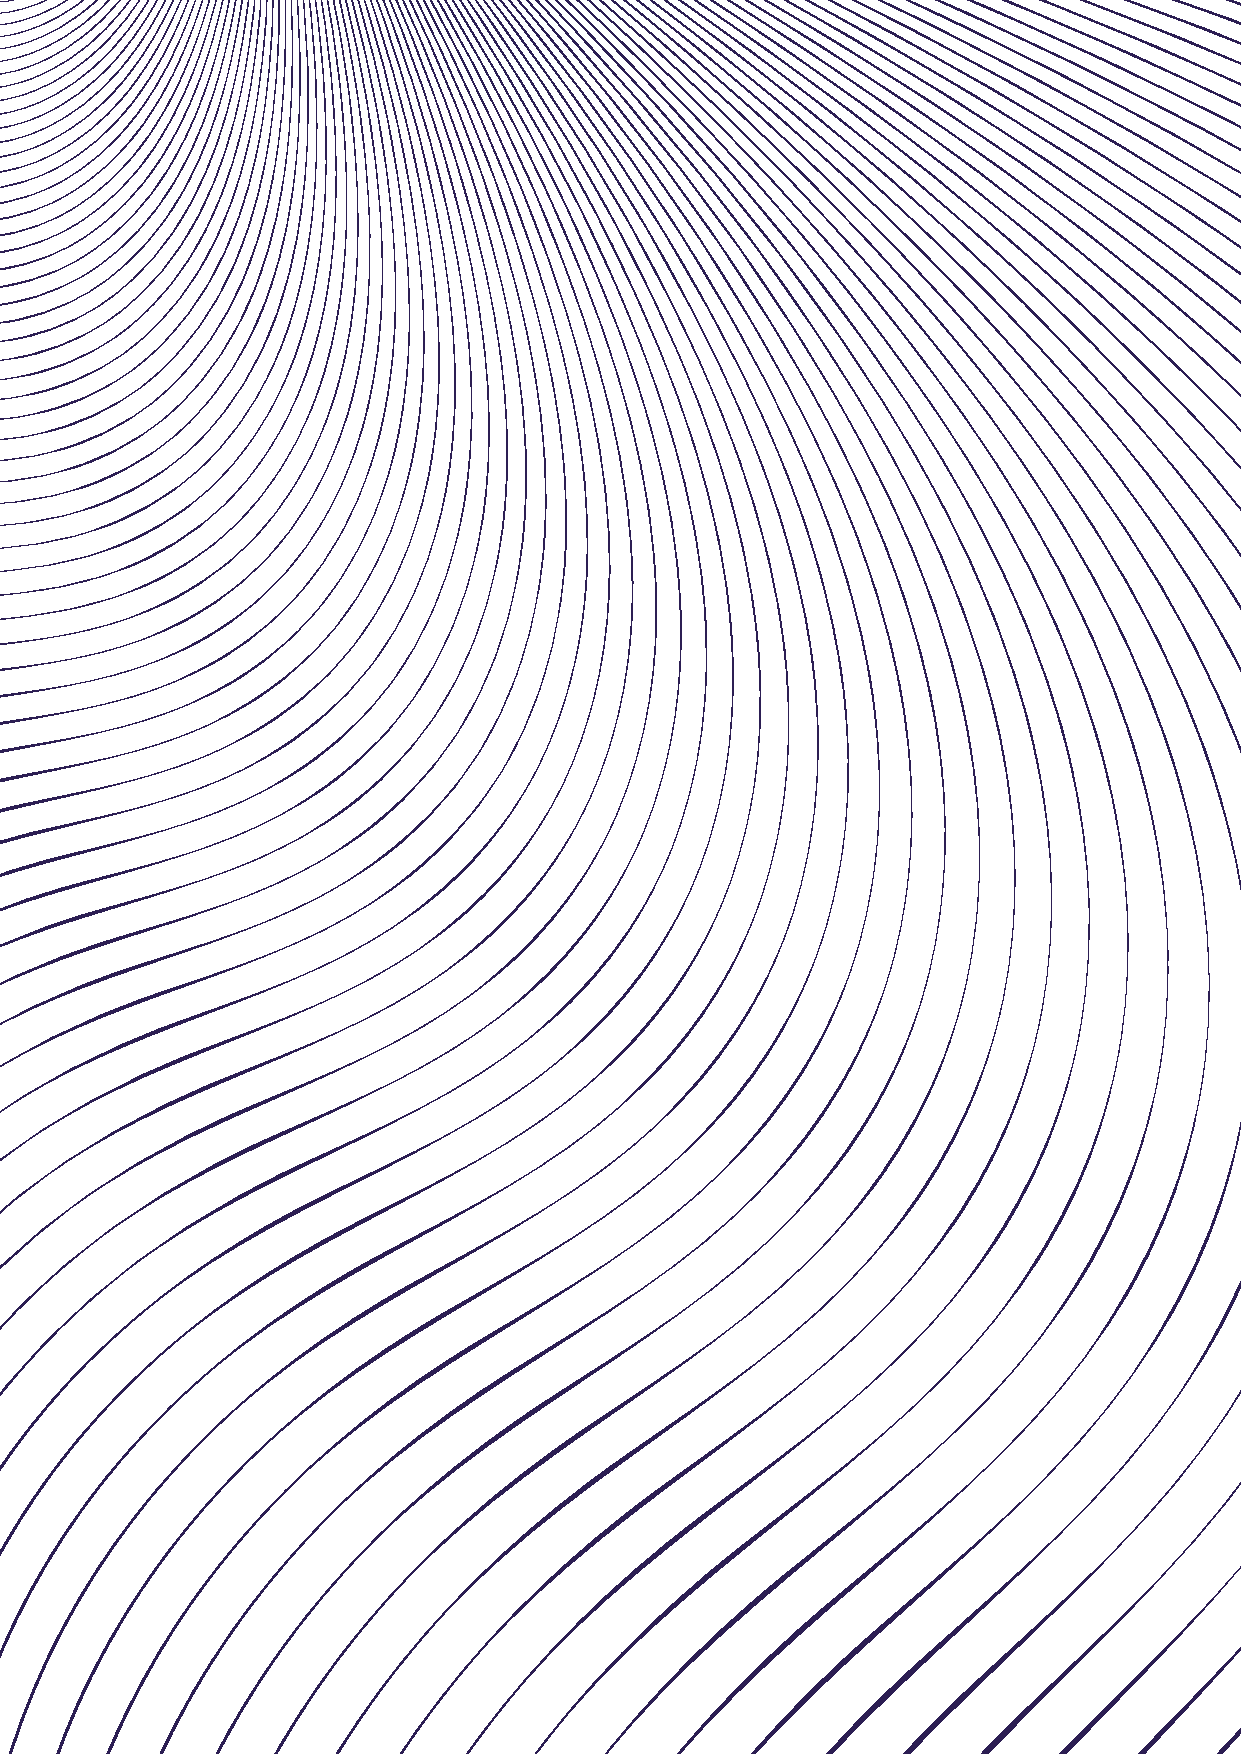
\includegraphics[width=\paperwidth,height=\paperheight]{AAUgraphics/aau_waves}}
    }
  \addtolength{\hoffset}{0.5\evensidemargin-0.5\oddsidemargin} %set equal margins on the frontpage - remove this line if you want default margins
  \noindent%
  {\color{white}\fboxsep0pt\colorbox{aaublue}{\begin{tabular}{@{}p{\textwidth}@{}}
    \begin{center}
    \Huge{\textbf{
      Dazel% insert your title here
    }}
    \end{center}
    \begin{center}
      \Large{
        A Programming Language for 
        
        Generating Top-Down Adventure Games% insert your subtitle here
      }
    \end{center}
    %% \vspace{0.2cm}
   \begin{center}
    {\large
      Christian Houmann, Ivik Hostrup, Patrick Østergaard% insert names separated by comma
    }\\
    \vspace{0.4cm}
    {\large
      \textit{Software, \authorname, 2021}% insert name of study, group number, year-month
    }
  \end{center}
   \vspace{0.2cm}
%% Comment this section in if you are doing Bachelor or Master Project   
%   \begin{center}
%     {\LARGE
%       %Bachelor Project
%       Master Project
%     }
%   \end{center}
  \end{tabular}}}
  \vfill
  \begin{center}
    
\includegraphics[width=0.2\paperwidth]{AAUgraphics/aau_logo_circle_en}% comment this line in for English version
    %
\includegraphics[width=0.2\paperwidth]{AAUgraphics/aau_logo_circle_da} %comment this line in for Danish version
  \end{center}
\end{titlepage}
\clearpage

\phantomsection
\pdfbookmark[0]{Titlepage}{titlepage}
\thispagestyle{empty}

\begin{singlespace} 
\setstretch{1.3}
\begin{minipage}[t]{0.48\textwidth}
    \vspace*{-25pt}			%\vspace*{-9pt}
    
\includegraphics[height=3.5cm]{AAUgraphics/aau_logo_en}
    \end{minipage}
    \hfill
    \begin{minipage}[t]{0.48\textwidth} {
        \small 
        \textbf{Software} \\
        Aalborg University \\
        https://www.aau.dk/
    }
\end{minipage}

\vspace*{1cm}

\begin{minipage}[t]{0.48\textwidth}
    \textbf{Title:} \\[5pt]\bigskip\hspace{2ex}
    Dazel
    
    \textbf{Project:} \\[5pt]\bigskip\hspace{2ex}
    P4-project
    
    \textbf{Project period:} \\[5pt]\bigskip\hspace{2ex}
    February 2021 - May 2021
    
    \textbf{Project group:} \\[5pt]\bigskip\hspace{2ex}
    \authorname %declare name in setup/macros.tex
    
    \textbf{Participants:} \\[5pt]\hspace*{2ex}
    Andreas Kamp Hansen \\\hspace*{2ex}
    Christian Bager Bach Houmann \\\hspace*{2ex}
    Ivik Lau Dalgas Hostrup \\\hspace*{2ex}
    John Hien Tri Nguyen \\\hspace*{2ex}
    Patrick Frostholm Østergaard \\\hspace*{2ex}
    Rasmus Solberg Collingwood Pyke \\\hspace*{2ex}
    
    \textbf{Supervisor:} \\[5pt]\hspace*{2ex}
    Giorgio Bacci
    
    \vspace*{0.5cm}
    
    \textbf{Page Numbers:} \pageref{bib:mybiblio} \\
    
    \textbf{Date of Completion:} \\[5pt]\hspace*{2ex}
    \today
\end{minipage}
\hfill
\begin{minipage}[t]{0.483\textwidth}
    \textbf{Abstract} \\[5pt]
    \fbox{\parbox{7cm}{\bigskip\small{The motivation for this project is to make game development and programming more accessible to beginners.
This report covers the design and implementation of the \dazel{} programming language.
We describe the process of designing the language based on research and our own experiences and preferences.
This includes designing the syntax using a context free grammar and formalizing the semantics.

To implement this, we started by generating a parser based on the formal grammar specification using ANTLR.
This gave us the foundation for implementing the subsequent phases of the \dazel{} compiler including building an abstract syntax tree, performing semantic analysis and generating intermediate models. 
Finally, we implemented an interpreter that interprets these models and generates the final result using the Unity game engine.
Along the way, we have performed several different types of tests to verify the correctness of our implementation.

The end product is a simple language, functional compiler and a simple prototype for generating top-down adventure games.\bigskip}}}
\end{minipage}

\vfill

{\scriptsize\itshape The content of the report is freely available, but publication (with source reference) may only take place in agreement with the authors.}

\end{singlespace}
\chapter*{Preface}
\thispagestyle{empty}

Here's the preface.\fxfatal{Write preface.}
\clearpage
\pdfbookmark[0]{Contents}{label:contents}
\tableofcontents
%Avoid page numbering before start of report
\thispagestyle{empty}
\addtocontents{toc}{\protect\thispagestyle{empty}}

% MAINMATTER
\pagestyle{fancy} %enable headers and footers again
\pagenumbering{arabic} %use arabic page numbering in the mainmatter
\setcounter{page}{0}%Reset page count

\chapter{Introduction} \label{chap:introduction}
Here is the introduction. The next chapter is \chapref{chap:analysis}.\\ % From macros.tex
\Chapref{chap:analysis} explains how to cite an external source.\\

Make sure to make custom commands in \texttt{macros.tex} to ensure homogeneous wording. Examples:
\begin{itemize}
    \item \sql\ (Some people might spell it like this: "sql")
    \item \sqldb
    \item \Ui\ / \ui\ (Some people might spell it like this: "user-interface", "ui" or "UI")
    \item \Frontend\ / \frontend\ (Some people might spell it like this: "front-end")
    \item \Backend\ / \backend
\end{itemize}

\section{How Does Sections, Subsections, and Subsections Look?}
Well, like this.
\subsection{This is a Subsection}
and this
\subsubsection{This is a Subsubsection}
and this.

\paragraph{A Paragraph}
You can also use paragraph titles which look like this.

\lipsum
\chapter{Problem Analysis} \label{chap:analysis}
Learning how to code is hard.
It is no wonder that the most viewed video on YouTube for the search term '\textit{learn programming}' has been viewed 23 million times\cite{LearnProgrammingYouTube}.
The video concerns itself with \textit{Python}, a language that is regarded as an easy to learn for beginners\cite{PythonBeginners}.

A common error, and source of frustration, for new programmers is syntax errors.
Other issues are types and confusing error outputs \cite{bosseWhyProgrammingDifficult2017}.
New programmers also have difficulties with the application of programming concepts.
This could be because learning isn't practical enough\cite{lahtinenStudyDifficultiesNovice2005}.
You have to program to learn how to program.

Is a simple language, like Python\cite{WhatPythonExecutive}, the solution for new programmers?
Research indicates that it might be. A simple language gives rise to fewer syntax errors as well as fewer logic errors.
Furthermore, learning a simpler language does not seem to hinder the learner when moving to a more complex language\cite{mannilaWhatSimpleLanguage2006}.


Knowing this, can a simple language be created which acts as a bridge to programming for beginners?
Before a more specific problem can be identified, we will get an overview of some existing solutions to this problem.

\section{Similar Solutions}
% ! See Notion -> Outline. We should have defined an initial problem which we can refer to. Just like I do below.
This section aims to give an overview of how other technologies attempt to solve a problem similar to ours. We decided to research these similar solutions such that we can draw inspiration from them.

\subsection{Scratch}\label{ScratchSection}
\begin{quote}
    ``\emph{A key goal of Scratch is to introduce programming to those with no previous programming experience.}'' - Maloney et al, 2010\cite{maloneyScratchProgrammingLanguage2010}
\end{quote}

Scratch\cite{ScratchImagineProgram} is the first programming language that comes to mind - and for good reason. At the time of writing, Scratch has 68 million registered users\cite{ScratchImagineProgramStatistics}. This makes it the most popular solution for a closely adjacent problem to ours. It also indicates that there is a desire to learn how to program through a largely visual and interactive platform.


% !! I have chosen to expand exhaustively on what makes Scratch stand out. It is, by far, the most popular and well-developed platform. They also provided a paper, which made it much more scientifically valid for us to use. There is much to learn from it. If we do not draw inspiration from any of the below features, we could (and perhaps, should) make this a bit shorter.
There are a few features which makes Scratch stand out as a platform to learn programming.
\begin{itemize}
    \item Scratch is always live. A user is not restricted from editing while their script is running. This helps users stay engaged in ``testing, debugging, and improving their projects.''\cite{maloneyScratchProgrammingLanguage2010}
    \item Scratch provides visual feedback to their users.\cite{maloneyScratchProgrammingLanguage2010}
    \item Scratch does not show error messages. Instead, it attempts error-recovery.\cite{maloneyScratchProgrammingLanguage2010}
    \item Scratchs' syntax consists of four types of blocks; command blocks, function blocks, trigger blocks, and control structure blocks.\cite{maloneyScratchProgrammingLanguage2010}
    \item There are only three data types; boolean, number, and string.\cite{maloneyScratchProgrammingLanguage2010}
    \item Concurrency, or multi-threading, is supported. A sprite can several things at once.\cite{maloneyScratchProgrammingLanguage2010}
\end{itemize}

\subsection{CodeCombat}\label{CodeCombatSection}
CodeCombat is similar to Scratch in that it aims to teach users how to program.
Their approaches are very different, though. CodeCombat is a programming game while Scratch is a programming language.

In CodeCombat, users are able to write code in JavaScript or Python\cite{CodeCombatCodingGames}. The user plays through a code-editor, writing lines of code which moves their character. It is similar to accessing their character through an API.

In CodeCombat, you learn about various programming concepts such as syntax, methods, parameters, loops, and variables through the levels in the game\cite{CodeCombatCodingGames}.

\subsection{Conclusion}
Both \secref{CodeCombatSection} and \secref{ScratchSection} present existing solutions that are designed to introduce users to programming.

They provide different approaches in order to achieve this. CodeCombat provides a representation of programming that is closer to writing code than Scratch, as Scratch provides blocks as an abstraction over textual code.
Another difference is how users are taught programming. Using Scratch, learning happens implicitly. There are no levels designed to teach you programming concepts - but there are tutorials. The primary focus is on building. CodeCombat, on the other hand, is more explicit in teaching the user programming concepts. Learning is necessary in order to progress through the levels.

% ! Should this section be rounded off more? I have given a generalized conclusion as this section should come before the problem definition. We can draw upon inspiration from these existing solutions there.
% ! I guess you could say that we draw inspiration from both. We, like Scratch, focus on world- and story-creation, which gives more freedom than the linear story of CodeCombat. We draw from CodeCombat in that we provide a textual way of creating.
% !! On the background of the existing solutions, we can draw some conclusions and narrow the problem down...
\section{Initial problem}\label{sec:initial_problem}
In the introduction to \chapref{chap:analysis} we asked whether it would be possible to design a simple language which would act as a bridge to programming for beginners.
Having examined some existing solutions to how beginners can be taught programming, a more specific problem can now be formulated.

In the simple programming language, inspiration should be drawn from what works in Scratch and CodeCombat. Furthermore, the language should serve as an attempt to both breathe fresh air onto the learning experience for beginners in addition to solving some of the problems that new programmers face.

Below is the proposed specification of such a language.

\begin{figure}[h]
    \vspace{0.5cm}
    \centering
    \begin{framed}
        A programming language with a simple syntax which resembles that of modern programming languages while promoting practical learning and providing visual feedback to the written code.
    \end{framed}
    \vspace{-0.5cm}
    \caption{Specification for the \dazel{} programming language}
    \label{fig:dazel_specification}
    \vspace{0.5cm}
\end{figure}

To create a language like \dazel{}, the language design must attempt to accommodate the specification as much as possible. \Secref{sec:scientific_research} presents research which will guide the design of \dazel{}.
% !! Now that the initial problem has been specified, we can bridge towards design...
\section{Studies on intuitive language design} \label{sec:scientific_research}
In this section, we discuss relevant scientific research on the difficulties of programming for beginners.
Later, we shall use this as a basis for various design decisions in \dazel{} such that we can make more
informed decisions about the language syntax and semantics.

In an investigation by Stefik et al.\cite{stefik_empirical_2011}, participants - all of whom were
programming novices - would use different programming languages to solve the same tasks so as to compare intuitiveness.
It was concluded that keywords having names that directly alluded to their purpose was important to the novices.
For example, the keyword \emph{repeat} was rated to be nearly seven times more intuitive to use than the keyword \emph{for}.
As language designers, such discoveries are important to take note of, as it emphasizes the importance of using intuitive words for language keywords.

A different investigation from 2019 about children and programming by Papavlasopoulou et al.\cite{papavlasopoulou_exploring_2019} discovered that
programming stereotypes exist, even among children.
In the study, it was found that many of the participating girls had no experience with programming, and that they believed it
to be an activity exclusively performed by "geeks".
To remedy this prejudice, the authors had the children develop storyboards in groups from which they would develop games using the
Scratch programming language.
This made the girls realize the potential of storytelling by programming video games, and it helped motivate them to learn programming.

This study highlights the importance of presenting not just the mathematical aspect of programming to novices, but also
showing them other uses, such as being able to develop entertainment.
It also shows that being able to tell a story makes learning programming more engaging for beginners.


A final investigation we would like to discuss is by Bosse et al.\cite{bosseWhyProgrammingDifficult2017}.
It followed different progamming courses and gathered data from the participants' diaries as well as through interviews with the teachers.
This investigation found that variable typing was quite troublesome for the participants, as they had trouble understanding when to use
types such as \texttt{double}, \texttt{float} or \texttt{int} to represent numbers. This also led to issues when using division, as participants
did not understand why the expression 1/2 yielded the integer 0 when they expected 0.5.
It was also found that functions and return types were difficult to grasp for the course participants, implying that basic mathematical
knowledge is an important prerequisite for learning programming, as both concepts are a major part of both mathematics and science in general.
Finally, the participants also had trouble understanding scope rules, which may suggest that language designers should consider how to be more explicit about scope rules in their language.


When we design our language in \chapref{chap:language_design}, we will use the conclusions from these studies to help us design a language that will suit our target demographic
as best as possible.

\chapter{Learning} \label{chap:analysis}


There are various factors, ways and methods for how humans can learn something effectively. 
This section will focus on how developing a game, can be a good way for new programmers to start programming and a better way for them to learn it as well.\newline

One key factor in order to learn something effectively is through deliberate practice (deliberate practice). The term \emph{deliberate practice} is refered to as when an "individual intentionally repeats an activity in order to improve performance". 
This means in order for new programmers to effectively learn to code, it is not enough to simply view/listen to a tutorial on programming, nor is it enough to rotely repeat a given task over and over again. Instead it indcludes deliberate practice for the learning individual. This requires attention, rehearsal and repetition. 
In order to achieve these 3 things, one may look at the role of interest has, as this is also a very important thing for promoting effective learning. In a study on the importance of interest in education, interest can be defined as "both a psychological state of attention and affect toward a particular object or topic, and an enduring predisposition to reengage over time" (interest attention).
In other words, in order for new programmers to learn something effectively, it is first and foremost important that they practice deliberately. This requires attention, in which it is important for the new programmers to have an interest in what they are practicing. 
Secondly deliberate practice also required repetition. As mentioned in the above quote, interest plays an important role in this aspect as well, since interest can make it easier for programmers to repeatedly program more and more over time, while their attention and focus are being directed at the task at hand.\newline

In chapter... it can be seen that there are a lot of new programmers who gets into programming by developing/wanting to develop games. This means there is a big interest for game development and it is something more and more people want to get into. And as it was established in this section, interest plays an important role for promoting effective learning.
Game development can therefor be a very good way for people to learn progamming. 

// evt skrive at det er grunden til at vi valge vores målgruppe er nybegyndere...

\chapter{Video games and computer interest} \label{chap:analysis}
In this section the relationship between video games, interest in computer science and game development is discussed. \newline

Research from Georgia Institute of Technology has shown a positive correlation between playing video games and the interest in computer science. The research included a survey which 1116 students participated in; the results shows that 43\% of student claim that playing games have increased their interest in computing by a lot. 
Even though the results from the study show a low interest in becoming a computer scientist (6.9\%), nearly 10\% (92 out of 1116 students) reported that playing video games sparked a “desire to make games”. 
This means that a fair number of young students has the desire to make games without necessarily being interesting in learning or studying computer science. Therefore, a simple and easy programming language that enables the user to quickly create and explore the possibilities in game development could be in demand.
As discussed in the previous section interest plays an important role in effective learning. Therefore learning a simple code language could be a good stepping stone to help understand a more complex languages.

\chapter{How to get more people starting with programming}\label{chap:analysis}

This section will focus on how to get more people  to start programming and what the best way to teach it is. \newline

Learning how to code is not easy, taking the first steps into this huge universe might seem like a daunting, if not intimidating task. All software is written in some kind of coding language and every coding language is unique, designed with a certain operating system, platform, coding style and intended use in mind. 
That is why many have a hard time starting to program because the coding world can be complicated and confusing to get into. It takes years of pratice to learn everything necessary to get beyond just a basic level where you can write short programs that work. It takes hours of practice.
There are plenty of free resources beginners can use to give themselves all the help they need. It can help them teach new techniques, and make the learning process fun and exciting. 
One of the most important ways before starting to program, is to find a reason to learn a programmming language. The answer can help determine which programming language should be used whetever it is to make a new indie game or making the newest application.
Another way to get the best learning expericence is to get a real book that you can follow along from beginning till the end. This will give more comprehensive introduction to coding than jumping around from topic to topic on a website. Another idea to start programming is to watch educational videos about nearly any coding related topic. 
It will give a more understanding of the topic and can be helping guidelines to the personal project a person want to make. 



  

\section{Studies on intuitive language design} \label{sec:scientific_research}
In this section, we discuss relevant scientific research on the difficulties of programming for beginners.
Later, we shall use this as a basis for various design decisions in \dazel{} such that we can make more
informed decisions about the language syntax and semantics.

In an investigation by Stefik et al.\cite{stefik_empirical_2011}, participants - all of whom were
programming novices - would use different programming languages to solve the same tasks so as to compare intuitiveness.
It was concluded that keywords having names that directly alluded to their purpose was important to the novices.
For example, the keyword \emph{repeat} was rated to be nearly seven times more intuitive to use than the keyword \emph{for}.
As language designers, such discoveries are important to take note of, as it emphasizes the importance of using intuitive words for language keywords.

A different investigation from 2019 about children and programming by Papavlasopoulou et al.\cite{papavlasopoulou_exploring_2019} discovered that
programming stereotypes exist, even among children.
In the study, it was found that many of the participating girls had no experience with programming, and that they believed it
to be an activity exclusively performed by "geeks".
To remedy this prejudice, the authors had the children develop storyboards in groups from which they would develop games using the
Scratch programming language.
This made the girls realize the potential of storytelling by programming video games, and it helped motivate them to learn programming.

This study highlights the importance of presenting not just the mathematical aspect of programming to novices, but also
showing them other uses, such as being able to develop entertainment.
It also shows that being able to tell a story makes learning programming more engaging for beginners.


A final investigation we would like to discuss is by Bosse et al.\cite{bosseWhyProgrammingDifficult2017}.
It followed different progamming courses and gathered data from the participants' diaries as well as through interviews with the teachers.
This investigation found that variable typing was quite troublesome for the participants, as they had trouble understanding when to use
types such as \texttt{double}, \texttt{float} or \texttt{int} to represent numbers. This also led to issues when using division, as participants
did not understand why the expression 1/2 yielded the integer 0 when they expected 0.5.
It was also found that functions and return types were difficult to grasp for the course participants, implying that basic mathematical
knowledge is an important prerequisite for learning programming, as both concepts are a major part of both mathematics and science in general.
Finally, the participants also had trouble understanding scope rules, which may suggest that language designers should consider how to be more explicit about scope rules in their language.


When we design our language in \chapref{chap:language_design}, we will use the conclusions from these studies to help us design a language that will suit our target demographic
as best as possible.

\chapter{Importance of Programming} \label{chap:importance_of_programming}

Humans have entered a digital age, as more and more stuff gets 
digitalized every year. This transition has been ongoing for a few 
generations, and the need for software cannot be understated. The \fxfatal{need source}
world runs on software, your coffee machine, television, car, mobile
phone, and the list goes on, not to mention that every single business 
and organization in the world needs an app or website. Most companies
need custom made applications or websites, and therefore a lot of coders
is needed.

This digital transition has made humans more dependant on technology than ever - 
and for a good reason. The year 2020 when the pandemic hit the world is a good example of that.
The pandemic changed the every day lives of a lot of people. Due to restrictions and curfew,
people from all over the world had to stay at home. This also applied to people 
who were studying or working as well. Business still had work that needed to be done,
students still had education they needed to finish. However, the world could not simply 
standby and wait for the pandemic to go over. 

In order to solve this problem,
various digital solutions have been used to prevent the world economy from receding.
Technology in form of video communication platforms such as Zoom and Microsoft Teams,
have allowed students to be able to stll receive teaching/lectures and study material online. 
Workers, who's work often consists of meetings and communication with other people,
have also been able to continue doing there work from home through video communication platforms. 
Restaurants and other businesses in the food industry have been able keep selling food, 
even with restrictions prohibiting customers to enjoy their food at the restaurant, 
they have shifted their sales to take away, where customers for example can order
food from their website or through an app such as Wolt. \newline


What do all these digital solutions have in common? They have all been created by 
some people programming them. Technology can help humans ease or solve these problems, 
but only if the machine or device have been programmed how to solve these problems. 
Zoom for example, would not have been able to allow people to have virtual meetings, 
if it had not been programmed to record each users webcam and microphone, and then output
it to each others devices. Wolt/restaurants could not have been able to manage
their orders online as effectively, if it was not for every step in the order process
being programmed - from displaying the restaurant's menu cart in the app, to make customers
able to order items from the menu and then send this information to Wolt workers that then 
deliver the orders. \newline

The takeaway from this is not that the the relevance of technology and programming 
only is due to the unexpected pandemic that occured,
but rather that the world and humans have - and will continue to face many problems post pandemic as well. Whether it is about gathering and analyzing data,
creating and improving automation such as in the production industry or even autonomous vechicles,
humans dependence and request for technology tbat ease their lives, will only continue
to grow and thus the importance of programming can be said to more important than ever.

\fxfatal{Need to answer "Do we need more programmers?"}
% include a bit statistical/factual data about actual needing demand for programmers/software engineers




\section{Similar Solutions}
% ! See Notion -> Outline. We should have defined an initial problem which we can refer to. Just like I do below.
This section aims to give an overview of how other technologies attempt to solve a problem similar to ours. We decided to research these similar solutions such that we can draw inspiration from them.

\subsection{Scratch}\label{ScratchSection}
\begin{quote}
    ``\emph{A key goal of Scratch is to introduce programming to those with no previous programming experience.}'' - Maloney et al, 2010\cite{maloneyScratchProgrammingLanguage2010}
\end{quote}

Scratch\cite{ScratchImagineProgram} is the first programming language that comes to mind - and for good reason. At the time of writing, Scratch has 68 million registered users\cite{ScratchImagineProgramStatistics}. This makes it the most popular solution for a closely adjacent problem to ours. It also indicates that there is a desire to learn how to program through a largely visual and interactive platform.


% !! I have chosen to expand exhaustively on what makes Scratch stand out. It is, by far, the most popular and well-developed platform. They also provided a paper, which made it much more scientifically valid for us to use. There is much to learn from it. If we do not draw inspiration from any of the below features, we could (and perhaps, should) make this a bit shorter.
There are a few features which makes Scratch stand out as a platform to learn programming.
\begin{itemize}
    \item Scratch is always live. A user is not restricted from editing while their script is running. This helps users stay engaged in ``testing, debugging, and improving their projects.''\cite{maloneyScratchProgrammingLanguage2010}
    \item Scratch provides visual feedback to their users.\cite{maloneyScratchProgrammingLanguage2010}
    \item Scratch does not show error messages. Instead, it attempts error-recovery.\cite{maloneyScratchProgrammingLanguage2010}
    \item Scratchs' syntax consists of four types of blocks; command blocks, function blocks, trigger blocks, and control structure blocks.\cite{maloneyScratchProgrammingLanguage2010}
    \item There are only three data types; boolean, number, and string.\cite{maloneyScratchProgrammingLanguage2010}
    \item Concurrency, or multi-threading, is supported. A sprite can several things at once.\cite{maloneyScratchProgrammingLanguage2010}
\end{itemize}

\subsection{CodeCombat}\label{CodeCombatSection}
CodeCombat is similar to Scratch in that it aims to teach users how to program.
Their approaches are very different, though. CodeCombat is a programming game while Scratch is a programming language.

In CodeCombat, users are able to write code in JavaScript or Python\cite{CodeCombatCodingGames}. The user plays through a code-editor, writing lines of code which moves their character. It is similar to accessing their character through an API.

In CodeCombat, you learn about various programming concepts such as syntax, methods, parameters, loops, and variables through the levels in the game\cite{CodeCombatCodingGames}.

\subsection{Conclusion}
Both \secref{CodeCombatSection} and \secref{ScratchSection} present existing solutions that are designed to introduce users to programming.

They provide different approaches in order to achieve this. CodeCombat provides a representation of programming that is closer to writing code than Scratch, as Scratch provides blocks as an abstraction over textual code.
Another difference is how users are taught programming. Using Scratch, learning happens implicitly. There are no levels designed to teach you programming concepts - but there are tutorials. The primary focus is on building. CodeCombat, on the other hand, is more explicit in teaching the user programming concepts. Learning is necessary in order to progress through the levels.

% ! Should this section be rounded off more? I have given a generalized conclusion as this section should come before the problem definition. We can draw upon inspiration from these existing solutions there.
% ! I guess you could say that we draw inspiration from both. We, like Scratch, focus on world- and story-creation, which gives more freedom than the linear story of CodeCombat. We draw from CodeCombat in that we provide a textual way of creating.


\chapter{Language design}
This chapter details the design of \dazel.
The language is intended to be a transitional language from visual programming to high-level language. Based on the problem analysis, it has been possible to specify the design for the user.
The target group is beginners in programming who are younger people. Therefore a programming language to make computer games has been built. This has been chosen as young people can relate more to video games as their hobby. \fxfatal{Kunne godt uddybes en del:
    "This has been chosen as young people can relate more to video games as their hobby" - skrev vi ikke lidt om det her i starten? måske lidt at hente derfra.
    Men i hvert fald en kilde på at understøtte påstanden. - John's review on PR}
This will help them to understand the principles of how a game should work more easily, and therefore be able to start programming. \fxfatal{Maybe give an example of what principles? - John's review on PR}
It was decided to develop a language inspired by the game "the Legend of Zelda: Link’s Awakening" into the programming language, as it is a familiar game with basic game terminologies.
This helps to set a framework for what the program language should be capable of.
In addition, "Unity" has been used as a program to test different functions to find out what could work well for the program language.

\section{Code examples}

\begin{lstlisting}[caption={Example screen}, label={lst:SampleScreen1},escapechar=|]
// ./Screens/SampleScreen1.txt
Screen SampleScreen1 
{
    Map 
    {
        Size(30, 24);

        Walls(Stone); 
        Floor(Grass);

        Line(TopLeft, TopRight, Cliff);
        Line([2, 2], [2, 4], Cliff);

        Square(position, size, Cliff);
        Square([8, 8], 4, Cliff);
    }

    OnScreenEntered
    {
        if Player.CompletedQuest(...) 
        {
            SetTile([4, 0], Stair);
        }
    }

    Entities
    {
        SpawnEntity(Skeleton1, [4, 4]).SetMovePattern(Square1);
    }
    
    Exits 
    {
        // Two different ways to create an exit
        // Specific tile(s) or whole screen side
        Exit1 = Exit([4, 0], SampleScreen2.Exit1);
        ScreenExit(Bottom, SampleScreen2);
    }
}
\end{lstlisting}

Code snippet~\ref{lst:SampleScreen1} shows an example of a screen. A screen represents a single area within the game, and each of the functions used within the Screen
define the layout, what happens as the screen is loaded, the entities that should be present as well as the exits of the level.
Objects such as Skeleton1 and the movement pattern Square1 on line 28 will be defined in a separate file.
The purpose of defining these separetely is to allow ease of reuseability and have a clear separation of concerns.

\section{Language design}
To start designing the programming language, we set out to specify a minimum viable product (MVP). We decided to start small but with expansion in mind.

\subsection{Keywords}\label{sec:keywords}
\Tabref{table:KeyWordsTable} introduces the reserved keywords in \dazel{}.  A convention has been introduced that defines all block-indicators to be denoted by an upper-case first character.

\begin{table}[h!]
    \centering
    \begin{tabular}{l|l}
    \textbf{Keyword}             & \textbf{Description}                                                                                                                                                                                                                                            \\ 
    \hline
    Player                       & \begin{tabular}[c]{@{}l@{}}A globally accessible reference\\ to the player. This allows the\\ programmer to create interactions \\involving the player's properties such \\as health or position.\end{tabular}  \\ 
    \hline
    Screen                       & \begin{tabular}[c]{@{}l@{}}Denotes a screen game object, which is a \\container for other blocks such as \\'Map', 'OnScreenEntered', 'Entities', \\and 'Exits'.\end{tabular}                                                                                          \\ 
    \hline
    Entity                       & \begin{tabular}[c]{@{}l@{}}Denotes an entity game object used to define the \\behavior of an entity.\end{tabular}                                                                                                                                                     \\ 
    \hline
    MovePattern                  & \begin{tabular}[c]{@{}l@{}}Denotes a move pattern game object which \\can be used to apply movement to\\entities.\end{tabular}                                                                                                                                        \\ 
    \hline
    Exits, ScreenExit, FloorExit & \begin{tabular}[c]{@{}l@{}}Denotes exits or transitions to other screens.\\These are usually triggered by player \\movement.\end{tabular}                                                                                                                       \\ 
    \hline
    Map                          & \begin{tabular}[c]{@{}l@{}}Denotes a map block which can be used\\to define a screen's size and its tile layout.\end{tabular}                                                                                                                                   \\ 
    \hline
    OnUpdate                     & \begin{tabular}[c]{@{}l@{}}Denotes an update block whose code is\\executed every frame.\end{tabular}                                                                                                                                                            \\ 
    \hline
    Data                         & \begin{tabular}[c]{@{}l@{}}Denotes a data block which can define\\properties such as health on entities.\end{tabular}                                                                                                                                           \\ 
    \hline
    Pattern                      & \begin{tabular}[c]{@{}l@{}}Denotes a pattern block which can be used\\to define specific movement patterns\\that may be reused across\\multiple entities.\end{tabular}                                                                                          \\ 
    \hline
    Entities                     & \begin{tabular}[c]{@{}l@{}}Denotes an entities block which can be\\used to define placement of entities on\\a given screen.\end{tabular}                                                                                                                        \\
    \hline
    until                        & \begin{tabular}[c]{@{}l@{}}Used to indicate that there is a condition\\for a repeat loop.\end{tabular}                                                                                                                                                          \\ 
    \hline
    or                           & Logical OR operator.                                                                                                                                                                                                                                            \\ 
    \hline
    and                          & Logical AND operator.                                                                                                                                                                                                                                                
    \end{tabular}
    \caption{Table explaining reserved keywords in \dazel}
    \label{table:KeyWordsTable}
\end{table}

\subsection{Built-in functionality}
Since we do not allow function definitions, we provide the programmer with a set of built-in functions that may be used to create their game. Explanations of these can be seen in \tabref{table:explanations_of_functions}.
In the table, we use \textbf{pos} to denote positions, which are arrays consisting of two elements where the first element is the x coordinate and the second element is the y coordinate.

\begin{longtable}{l|l}
    \multicolumn{1}{c|}{\textbf{\textit{Function}}}                                                                                                                                                                                                                                                  & \multicolumn{1}{c}{\textbf{\textit{Parameters}}}                                                                                                                                                                                                                                                                           \endfirsthead 
    \hline
    \begin{tabular}[c]{@{}l@{}}\textbf{Size(x, y):~}Sets the size of the map.\\\textbf{Return type:} void\\\textbf{Example:} Size(30, 24)\end{tabular}                                                                                                                                               & \begin{tabular}[c]{@{}l@{}}\textbf{x (int):} The width of the map in tiles.\\\textbf{y (int):~}The height of the map in tiles.\end{tabular}                                                                                                                                                                                \\ 
    \hline
    \begin{tabular}[c]{@{}l@{}}\textbf{Walls(tile):} Sets the outermost\\tiles on each side of the map to \\a certain tile type.\\\textbf{Return type:} void\\\textbf{Example:} Walls("Stone.png")\end{tabular}                                                                                      & \begin{tabular}[c]{@{}l@{}}\textbf{tile (string):} The name of the image file\\for the tile.\end{tabular}                                                                                                                                                                                                                  \\ 
    \hline
    \begin{tabular}[c]{@{}l@{}}\textbf{Floor(tile):\textit{~}}Sets the floor layer of each\\tile to be of a certain tile type.\\\textit{}\textbf{Return type:} void\\\textbf{Example:~}Floor("Grass.png")\end{tabular}                                                                               & \begin{tabular}[c]{@{}l@{}}\textbf{tile (string):} The name of the image file \\for the tile.\end{tabular}                                                                                                                                                                                                                 \\ 
    \hline
    \begin{tabular}[c]{@{}l@{}}\textbf{Line(pos1, pos2, tile):} Creates a line \\of a certain tile type.\\Takes two coordinates denoting start\\and end, as well as the desired tile type\textit{.}\\\textbf{Return type:} void\\\textbf{Example:} Line([2, 2], [2, 4], "Stone.png")\end{tabular}      & \begin{tabular}[c]{@{}l@{}}\textbf{pos1 (\textbf{Array}), pos2 (\textbf{Array}):} The start and\\end positions of the line.\\\textbf{tile(string):} The name of the image file\\for the tile.\end{tabular}                                           \\ 
    \hline
    \begin{tabular}[c]{@{}l@{}}\textbf{Square(pos, size, tile):~}Creates a \\square of a certain tile type.\\Takes a coordinate for the center \\position, a size and a tile type.\\\textbf{Return type:} void\\\textbf{Example:} Square([8, 8], 4, "Stone.png")\end{tabular}                       & \begin{tabular}[c]{@{}l@{}}\textbf{pos (\textbf{Array}):~}The position of the center\\of the square.\\\textbf{size (int):} An integer denoting the size of\\the square.\\\textbf{tile (string):} The name of the image file\\for the tile.\end{tabular}  \\ 
    \hline
    \begin{tabular}[c]{@{}l@{}}\textbf{MoveLeft()}\\\textbf{Return type:} void\end{tabular}                                                                                                                                                                                                          & \begin{tabular}[c]{@{}l@{}}Moves an entity one tile left.\\Used when specifying move patterns.\end{tabular}                                                                                                                                                                                                                \\ 
    \hline
    \begin{tabular}[c]{@{}l@{}}\textbf{MoveUp()}\\\textbf{Return type:} void\end{tabular}                                                                                                                                                                                                            & \begin{tabular}[c]{@{}l@{}}Moves an entity one tile up.\\Used when specifying move patterns.\end{tabular}                                                                                                                                                                                                                  \\ 
    \hline
    \begin{tabular}[c]{@{}l@{}}\textbf{MoveDown()}\\\textbf{Return type:} void\end{tabular}                                                                                                                                                                                                          & \begin{tabular}[c]{@{}l@{}}Moves an entity one tile down.\\Used when specifying move patterns.\end{tabular}                                                                                                                                                                                                                \\ 
    \hline
    \begin{tabular}[c]{@{}l@{}}\textbf{MoveUp()}\\\textbf{Return type:}\textit{ void}\end{tabular}                                                                                                                                                                                                   & \begin{tabular}[c]{@{}l@{}}Moves an entity one tile up.\\Used when specifying move patterns.\end{tabular}                                                                                                                                                                                                \\ 
    \hline
    \begin{tabular}[c]{@{}l@{}}\textbf{PlayerInAggroRange()}\\\textbf{Return type:} bool\end{tabular}                                                                                                                                                                                                & \begin{tabular}[c]{@{}l@{}}Returns a boolean indicating whether \\the player is within the\textasciitilde{}aggro range of a \\given entity.\\Can only be called within the scope of\\an entity.\end{tabular}                                                                                                               \\ 
    \hline
    \begin{tabular}[c]{@{}l@{}}\textbf{Exit(pos, screen): }Creates an exit at\\the given position which takes the\\player to the specified screen when\\interacted with.\\\textbf{\textbf{Return type:}}~\textit{Exit}\end{tabular}                                                                  & \begin{tabular}[c]{@{}l@{}}\textbf{pos (\textbf{Array}):}~The position at which to\\place the exit.\\\textbf{screen~\textbf{\textbf{\textbf{(Screen):~}}}}The identifier of the \\screen to connect the exit to.\end{tabular}                           \\ 
    \hline
    \begin{tabular}[c]{@{}l@{}}\textbf{ScreenExit(dir, screen):} Creates a\\screen exit in a given direction such\\that the player is taken to a different\\screen when walking off-screen in the\\specified direction.\\\textbf{\textbf{\textbf{\textbf{Return type:}}}}~\textit{Exit}\end{tabular} & \begin{tabular}[c]{@{}l@{}}\textbf{dir (Direction): }The direction the player \\must walk off-screen to trigger the exit.\\\textbf{\textbf{screen (Screen):}}~The identifier of the \\screen to connect the exit to.\end{tabular}                                                                                          \\ 
    \hline
    \begin{tabular}[c]{@{}l@{}}\textbf{SpawnEntity(entity, pos):} Spawns the\\given entity at the given position.\\\textbf{Return type:} \textit{Entity}\end{tabular}                                                                                                                                & \begin{tabular}[c]{@{}l@{}}\textbf{\textbf{entity (Entity): }}The identifier of the entity to \\spawn.\\\textbf{pos (Array):}~The position at which to\\spawn the entity.\end{tabular}                                                                    \\                                                                   
    \caption{Explanations of built-in functionalities}
    \label{table:explanations_of_functions}
\end{longtable}

\subsection{Statement Level Control Structures}
Users can change execution flow using control structures. These are if-statements and repeat-statements.
\subsubsection{If statements}
If statements are selection statements. These provide the means of choosing between two or more execution paths in a program\cite{sebesta_concepts_2016}.

In Dazel, if-statements are followed by an expression and then curly braces, which open a new scope. The statements within this scope are executed if the expression holds true.

\begin{lstlisting}[caption={Example of an if statement}, label={lst:ifexpression},escapechar=|]
if <expression>|\label{lst:exp}|
{
    Code...
}
\end{lstlisting}

In \ref{lst:ifexpression} on line \ref{lst:exp},  \verb|<expression>| denotes a placeholder expression.

\subsubsection{Repeat loops}
Repeat loops are iterative statements.

\begin{lstlisting}[caption={Example of loops}, label={lst:loops},escapechar=|]
repeat until <var> == 10|\label{lst:repeatuntil}|
{
    Code...
}

repeat forever|\label{lst:repeatforever}|
{
    Code...
}
\end{lstlisting}\fxfatal{Specify order of evaluation - once we've figured it out. See feedback 17/03}

In \ref{lst:loops} on line \ref{lst:repeatuntil}, \verb|<var>| denotes an arbitrary variable. It is expected that the expression will evaluate to true, otherwise the loop does the same as the \verb|repeat forever| loop on line \ref{lst:repeatforever}.

The \verb|repeat forever| loop repeats forever - or until the running instance terminates.
The \verb|repeat until| loop repeatedly executes the code in the scope immediately below it until the given expression evaluates to \verb|true|.
\subsection{Operator symbols}
\fxfatal{Work in progress. Should this be here?}
See \tabref{table:operatorsymbols}.

\begin{table}[h!]
    \centering
    \begin{tabular}{ |c|c|c||c|c|c|c| }
        \hline
        \textbf{Category} & \textbf{Operator} & \textbf{Associativity} & \texttt{Number} & \texttt{String} & \texttt{Boolean} & \texttt{Tile} \\                              
        \hline

        \multirow{6}{*}{Relational} 
        & \texttt{<}
        & $\rightarrow$ 
        & Type1 
        & Type2 
        & Type3 
        & Type4 
        \\
        
         
        & \texttt{>} 
        & $\rightarrow$ 
        & Type1 
        & Type2 
        & Type3 
        & Type4 
        \\

        
        & \texttt{==} 
        & $\rightarrow$ 
        & Type1 
        & Type2 
        & Type3 
        & Type4 
        \\

         
        & \texttt{!=} 
        & $\rightarrow$ 
        & Type1 
        & Type2 
        & Type3 
        & Type4 
        \\

         
        & \texttt{>=} 
        & $\rightarrow$ 
        & Type1 
        & Type2 
        & Type3 
        & Type4 
        \\

         
        & \texttt{<=} 
        & $\rightarrow$ 
        & Type1 
        & Type2 
        & Type3 
        & Type4 
        \\\hline

        \multirow{2}{*}{Logic}
        & \texttt{and} 
        & $\rightarrow$ 
        & Type1 
        & Type2 
        & Type3 
        & Type4 
        \\
 
        & \texttt{or} 
        & $\rightarrow$ 
        & Type1 
        & Type2 
        & Type3 
        & Type4 
        \\\hline
        
        Assignment 
        & \texttt{=}
        & $\leftarrow$ 
        & Type1 
        & Type2 
        & Type3 
        & Type4 
        \\\hline
        
        \multirow{4}{*}{Arithmetic} 
        & \texttt{+}
        & $\rightarrow$ 
        & Type1 
        & Type2 
        & Type3 
        & Type4 
        \\
        
         
        & \texttt{-}
        & $\rightarrow$ 
        & Type1 
        & Type2 
        & Type3 
        & Type4 
        \\
         
        & \texttt{*} 
        & $\rightarrow$ 
        & Type1 
        & Type2 
        & Type3 
        & Type4 
        \\
         
        & \texttt{/}
        & $\rightarrow$ 
        & Type1 
        & Type2 
        & Type3 
        & Type4 
        \\\hline
    \end{tabular}
    \caption{Operation symbols}
    \label{table:operatorsymbols}
\end{table}

\fxfatal{Fix types. Depends on implementation.}
\subsection{Context-Free Grammar Derivations}
There are two types of derivations; leftmost- and rightmost-derivations\cite{sebesta_concepts_2016}.

A \textit{leftmost derivation} is where the leftmost nonterminal symbol is replaced at each step of the derivation.

A \textit{rightmost derivation} is where the rightmost nonterminal is replaced at each step of the derivation.

Typically, bottom-up parsing algorithms use rightmost derivations in reverse. These are the LR parser and its variations. Likewise, most top-down parsers use leftmost derivations - this being the LL parser and its variations.
\subsection{Methods}
\subsection{Variables}

Variables in programming, also called a program variable, is a way of creating an abstraction of one or more memory cells.
In \cite{sebesta_concepts_2016}, a variable is characterized as a sextuple consisting of the attributes:

\begin{itemize}
    \item Name
    \item Address
    \item Type
    \item Value
    \item Lifetime
    \item Scope
\end{itemize}

In the following sections we will describe the basic theory behind each of the items, in the list above, and how we have chosen to approach them for our language design for \dazel{}.

\subsubsection*{Address, lifetime and values of variables}
Since \dazel{} will be translated to C\#, the addressing and lifetime of variables is primarily handled by the .NET runtime,
however we can influence it through the scope rules described in \secref{sec:semantics}.
In doing so, we can ensure that no two variables share the same address as long as they are declared within different scopes.
It is also worth noting that, while our language dictates the actual value of a variable, its memory allocation is still managed by the .NET runtime.

\subsubsection*{Name}

Variable names in a programming language is a string of characters used to identify an entity in the program\cite{sebesta_concepts_2016}. A name can be defined to be consisting of either capital letters,
lower case letters, some symbols or a mixture of all.

Specifically for our language design we have decided that a variable name can be constructed with the following rules:

\begin{itemize}
    \item A name can have capital letters
    \item A name can have lower case letters
    \item A name can start with a capital letter, followed by lower case letters
    \item A name can start with lower case letter(s) and have a single or more letters be capital following the first letter
    \item A name can have an arbitrary mixture of capital and lower case letters
    \item A name can end with an underscore symbol, but not start with an underscore symbol
    \item The is no specified limit on the length of the name
\end{itemize}

The list of rules mentioned can be simplified using the regular expression: [a-zA-Z][a-zA-Z\_0-9]*. Any construction of a variable outside of these rules will be considered
a non-valid construction.

How variables are defined in relation to their scope and type will be discussed in the description of the language semantics in \secref{sec:semantics}.

\subsubsection*{Member access}
In order to access properties within other objects, we have decided to include a member access functionality similar to what might be seen in a
object oriented language. Member access in \dazel{} provides the ability to access all user defined game objects, including screens, entities and move patterns as well
as built-in objects such as the player. To access a game object, one simply writes its identifier. To then access a property of the game object, one then writes
a dot, followed by the identifier of the desired property.

This is illustrated in code \snipref{lst:SampleScreen1} on line 47. In this example, the exit property with the identifier \texttt{Exit1} of \texttt{SampleScreen2} is accessed.
The effect of this is that the property in question becomes the value passed into the actual parameter of the \texttt{Exit} function call.


\subsection{Expressions}
A major part of any programming language is expressions of which there are several types.
In the following, we will introduce these and discuss their relevance to \dazel{}.

\subsubsection*{Arithmetic expressions}
Arithmetic expressions are basic mathematical expressions. 
They consist of operators, operands, and function calls. 
Operators can either be unary, binary or ternary meaning they have either one, two or three operands.
Finally, binary operators are usually infix, meaning they appear between operands.

In \dazel{}, tiles on screens are placed on a grid with the bottom left corner being located at (0, 0) and only growing positively.
Because of this, the language is only concerned with positive numbers, and consequently it exclusively features a variety of binary operators. 

- arithmetic Expressions
- operator evaluation order
	- precedence
	- associativity
	- parantheses
	- side effects
- relational expressions
- boolean expressions

\subsection{Language Grammar} \label{langGram}

In this section we will describe how to formally specify a language using constructs such as Backus-Naur form (BNF), Extended Backus-Naur form(EBNF).
Following these two topics we will introduce the concept of derivation, and which type of derivation we have chosen for our language. 
Finally, we will give a justification for this choice as well as concrete examples of how all the previously mentioned elements are represented in our language.

\subsection{Backus-Naur form}

Backus-Naur form was a an evolution of a formal notation used to describe the language ALGOL 58, introduced by John Backus in 1959. The evolution happened as a result of modifications
made to this notation by Peter Naur in 1960, when he was describing ALGOL 60. Hence why the notation became known as Backus-Naur form (BNF)\cite{sebesta_concepts_2016}. 

As alluded to, BNF is used as a formal notation to describe the language, or more specifically its grammar. The construction of this grammar is made up of a collection of production rules that are formed as shown in the example (indsæt eksmpel).

In (forrige indsatte figur) there is a left hand side (LHS) and a right hand side (RHS), separated by an arrow. The LHS is a variable, also called the abstraction, that is being defined and the RHS is the definition.
This definition on the RHS consists of non-terminals and terminals. A non-terminal is a variable (sometimes called a symbol) that is an abstraction that have references to other abstractions. 
These non-terminal variables can have multiple distinct definitions each being a possible form of the syntax. If a non-terminal has multiple definitions these can either be represented as multiple 
rules as seen in fig.. or as a single rule where each definition is seperated by an OR operator: '|'. Terminals correlates to a piece of the output, as shown in figure (indsæt fig). 
Terminals are also referred to as lexemes and tokens\cite{sebesta_concepts_2016}. 

\subsection{Extended Backus-Naur form}

Due to some people experiencing inconveniences, BNF has seen several different extensions.
These extended versions are commonly referred to as Extended BNF or just EBNF. 
EBNF is not any more powerful than BNF, rather it simply adjusts and adds to the syntax in an attempt to make it more readable.
Whether EBNF succeeds in that regard is completely subjective. 

Most versions of ENBF usually include three extensions:
- The use of square brackets to denote and optional part of the right-hand side of a production
- The use of curly brackets to indicate that the enclosed part may be iterated any number of times
- The use of the OR operator, |, to denote multiple-choice options for a production

Despite there being a standardized version of EBNF, it is rarely ever used. 
Whichever version a language designer decides to use is up to preference.

\subsection{Derivation}


\subsection{Justification}


\subsection{Member Access}
\section{Semantics for Dazel} \label{sec:semantics}

In this section we will be presenting, in an informal manner, the semantics of \dazel{}.
Firstly, we will present the type rules which is then followed by a presentation of the scope rules.

\subsection{Type Rules}

When designing a compiler, decisions have to be made concerning how you approach type checking.
Type checking can be divided into two categories, each of which have drawbacks and benefits. The categories are:

\begin{enumerate}
    \item \textit{Strong} versus \textit{Weak} types
    \item \textit{Static} versus \textit{Dynamic} types
\end{enumerate}

\subsubsection*{Strong and weak typing}
Strong and weak typing relates to how the type of a given variable can be determined at either run time or compile time.
Strong typing implies that the compiler is able to detect all the incorrect uses of variables that would otherwise result in type errors or illegal operations.
Weak typing implies that types will automatically be converted from one type to another or that type rule enforcement can easily be subverted.
For example, using a string in a numeric context will convert it to the string's numerical representation\cite{sebesta_concepts_2016}.

\subsubsection*{Static and dynamic typing}
Static typing means that the type is statically bound to the \emph{variable} and that types are checked at compile time.
In contrast, dynamic typing is where the type is bound to the \emph{value} and that the type is checked at run time\cite{sebesta_concepts_2016}.

The type of a variable can also either an implicit or explicit declaration.
The type then determines the value range and the set of operations available to this variable.

\subsection*{Type rules in \dazel{}}
\dazel{} has implicitly declared strong types.
This means the programmer does not need to explicitly define the type of every variable, however, once declared, a variable
cannot dynamically change type.
For example, as can be seen in \snipref{lst:IllegalAssignment}, \texttt{Exit1} is declared to be of type \texttt{Exit}, so it cannot be assigned to an integer afterwards.

\begin{lstlisting}[language=CSharp, caption={Example of an illegal assingment}, label={lst:IllegalAssignment},escapechar=|]
// ./Screens/SampleScreen1.txt
Screen SampleScreen1 
{
    Exits 
    {
        Exit1 = Exit([4, 0], SampleScreen2.Exits.Exit1);
        Exit1 = 1; // Not legal because Exit1 has type Exit
    }
}
\end{lstlisting}

The decision to use this system is based on the fact that strongly typed languages offer greater safety, however being required to
specify the type of each variable as part of its declaration is often confusing to beginners as mentioned in \secref{sec:scientific_research}.
Therefore, it was decided to go with a hybrid approach.

In addition, we decided to include four different types with corresponding array-types. These will be implicitly declared.

\begin{multicols}{3}
    \begin{enumerate}
        \item Numbers\label{item:numbertype}
        \item Booleans\label{item:booleantype}
        \item Strings\label{item:stringtype}
        \item Tiles\label{item:tiletype}
        \item Arrays*\label{item:arraytype}
    \end{enumerate}
\end{multicols}

\ref{item:numbertype} should denote both integer and floating point types. The actual type will be determined through context. \ref{item:booleantype} will be used for conditional expressions and control flow.
\ref{item:stringtype} will be used for naming.
\ref{item:tiletype} is an important type: it is the type behind every tile in the generated games.
\ref{item:arraytype} means that every type in the list will have a corresponding array type. This is to say that arrays are parametric — for example, an array could be an array of numbers.

\subsection*{Dynamic and static binding}
A variable must first be bound to a data type before it can be used in the program. 
This is called a binding and, depending on the language, it can either be dynamic or static.
\textit{Dynamic binding} is when the type of a variable is determined at runtime. 
\textit{Static binding} is when the type of a variable can be determined during compilation as all the necessary information is present in the source code \cite{sebesta_concepts_2016}.

\dazel{} uses static binding, as types are determined while the source code is compiled. When a variable is initially declared, it is assigned a type before the code is run.

\subsection{Scope Rules}
In this section we describe different types of scope rules, specifically static scopes, block scopes and dynamic scopes.
We will ultimately use this to determine the best fit for \dazel{}.

\subsubsection{Static Scopes}
\textit{Static scoping} is the act of binding names to nonlocal variables such that the scope of a variable
can be determined prior to program execution. This way, one can determine the type of every variable via the source code.
Static-scoped languages can be split into two categories: those that allow sub-programs to be nested and those that do not.
The former creates nested static scopes while the latter only creates nested scopes through nested class definitions and blocks.
Static scope rules are commonly used in modern languages due to their emphasis on static type checking\cite{sebesta_concepts_2016}.

\subsubsection{Dynamic Scopes}
In contrast to static scoping, variables declared in languages with \textit{dynamic scoping} are determined at runtime through the calling sequence of subprograms.

\begin{lstlisting}[language=CSharp, caption={Example of dynamic scoping}, label={lst:DynamicScopeExample}]
function main() {
	function nested1() {
		var x = 7;
	}
	
	function nested2() {
		var y = x;
	}

	var x = 3; 
}
\end{lstlisting}

In snippet \ref{lst:DynamicScopeExample}, assuming that dynamic scoping rules apply, the meaning of the identifier \texttt{x} cannot be determined at compile time.
Specifically, the declaration of an identifier is first searched for in the local function.
If no declaration for \texttt{x} is found, the search continues to the function's caller, its \textit{dynamic parent}, and so on up the call-stack\cite{sebesta_concepts_2016}.

\subsubsection{Blocks}
\textit{Blocks} serve as way to declare new static scopes within executable code.
This allows variables declared within a block to be local to that scope, meaning they cannot be accessed from outside the scope.
However, nested blocks can still access variables from outer scopes.
A variable declared within a block is allocated when the block is entered and deallocated when it is exited\cite{sebesta_concepts_2016}.

\subsubsection{Choice of Scope}
Due to the nature of action maps in games, we decided to use block scopes in order to separate the elements found within a screen.
In particular, a screen on the map is defined by a block containing nested blocks that describe the map's layout, its exits and the entities that spawn within the given screen.
For instance, the tilemap layout of a screen would be defined in a \texttt{Map} block containing definitions for tile placements.
This separation of screen elements made sense as it decouples the different parts of a screen by default.

\subsection{Context-Free Grammar Derivations}
There are two types of derivations; leftmost- and rightmost-derivations\cite{sebesta_concepts_2016}.

A \textit{leftmost derivation} is where the leftmost nonterminal symbol is replaced at each step of the derivation.

A \textit{rightmost derivation} is where the rightmost nonterminal is replaced at each step of the derivation.

Typically, bottom-up parsing algorithms use rightmost derivations in reverse. These are the LR parser and its variations. Likewise, most top-down parsers use leftmost derivations - this being the LL parser and its variations.
\subsection{Methods}
\subsection{Scope}
In this section we describe different types of scope rules, specifically static scopes, block scopes and dynamic scopes.
We will ultimately use this to determine the best fit for \dazel{}.

\subsubsection{Static Scopes}
Originally introduced by ALGOL 60, \texttt{static scoping} is the act of binding names to nonlocal variables such that the scope of a variable
can be determined prior to program execution. This way, one can determine the type of every variable via the source code.
Static-scoped languages can be split into two categories: those that allow sub-programs to be nested and those that do not.
The former creates nested static scopes while the latter only creates nested scopes through nested class definitions and blocks. 
Static scope rules are quite commonly used in modern languages due to their emphasis on static type checking.\cite{sebesta_concepts_2016}

\subsection{Dynamic Scopes}
In stark contrast to static scoping, variables declared in languages with \texttt{dynamic scoping} are determined at runtime through the calling sequence of subprograms.

\begin{lstlisting}[caption={Example of dynamic scoping}, label={lst:DynamicScopeExample}]
function main() {
	function nested1() {
		var x = 7;
	}
	
	function nested2() {
		var y = x;
	}

	var x = 3;
}
\end{lstlisting}

In listing \ref{DynamicScopeExample}, assuming that dynamic scoping rules apply, the meaning of the identifier \texttt{x} cannot be determined at compile time.
Specifically, the declaration of an identifier is first searched for in the local function. 
If no declaration for \texttt{x} is found, the search continues to the function's caller, its \texttt{dynamic parent}, and so on up the call-stack.\cite{sebesta_concepts_2016}

\subsubsection{Blocks}
The powerful concept of \texttt{block scoping} allows specific sections of code called blocks to have their own localized variables. 
Variables declared within a block are local, meaning they cannot be accessed from outside the scope. However, nested blocks can still access variables from outer scopes.
A variable declaed within a block is allocated when the block is entered and deallocated when it is exited.\cite{sebesta_concepts_2016}

\subsubsection{Choice of Scope}
Due to the nature of action maps in games, we decided to use block scopes in order to separate the elements found within a screen. 
In particular, a screen on the map is defined by a block containing nested blocks that describe the maps layout, its exits and the entities that spawn within the given screen.
For instance, the tilemap layout of a screen would be defined in a \texttt{Map} block containing definitions for tile placements.
This separation of screen elements made sense as it achieves decoupling between the different parts of a screen by default. 

\subsection{Variables}

Variables in programming, also called a program variable, is a way of creating an abstraction of one or more memory cells.
In \cite{sebesta_concepts_2016}, a variable is characterized as a sextuple consisting of the attributes:

\begin{itemize}
    \item Name
    \item Address
    \item Type
    \item Value
    \item Lifetime
    \item Scope
\end{itemize}

In the following sections we will describe the basic theory behind each of the items, in the list above, and how we have chosen to approach them for our language design for \dazel{}.

\subsubsection*{Address, lifetime and values of variables}
Since \dazel{} will be translated to C\#, the addressing and lifetime of variables is primarily handled by the .NET runtime,
however we can influence it through the scope rules described in \secref{sec:semantics}.
In doing so, we can ensure that no two variables share the same address as long as they are declared within different scopes.
It is also worth noting that, while our language dictates the actual value of a variable, its memory allocation is still managed by the .NET runtime.

\subsubsection*{Name}

Variable names in a programming language is a string of characters used to identify an entity in the program\cite{sebesta_concepts_2016}. A name can be defined to be consisting of either capital letters,
lower case letters, some symbols or a mixture of all.

Specifically for our language design we have decided that a variable name can be constructed with the following rules:

\begin{itemize}
    \item A name can have capital letters
    \item A name can have lower case letters
    \item A name can start with a capital letter, followed by lower case letters
    \item A name can start with lower case letter(s) and have a single or more letters be capital following the first letter
    \item A name can have an arbitrary mixture of capital and lower case letters
    \item A name can end with an underscore symbol, but not start with an underscore symbol
    \item The is no specified limit on the length of the name
\end{itemize}

The list of rules mentioned can be simplified using the regular expression: [a-zA-Z][a-zA-Z\_0-9]*. Any construction of a variable outside of these rules will be considered
a non-valid construction.

How variables are defined in relation to their scope and type will be discussed in the description of the language semantics in \secref{sec:semantics}.

\subsubsection*{Member access}
In order to access properties within other objects, we have decided to include a member access functionality similar to what might be seen in a
object oriented language. Member access in \dazel{} provides the ability to access all user defined game objects, including screens, entities and move patterns as well
as built-in objects such as the player. To access a game object, one simply writes its identifier. To then access a property of the game object, one then writes
a dot, followed by the identifier of the desired property.

This is illustrated in code \snipref{lst:SampleScreen1} on line 47. In this example, the exit property with the identifier \texttt{Exit1} of \texttt{SampleScreen2} is accessed.
The effect of this is that the property in question becomes the value passed into the actual parameter of the \texttt{Exit} function call.


\subsection{Expressions}
A major part of any programming language is expressions of which there are several types.
In the following, we will introduce these and discuss their relevance to \dazel{}.

\subsubsection*{Arithmetic expressions}
Arithmetic expressions are basic mathematical expressions. 
They consist of operators, operands, and function calls. 
Operators can either be unary, binary or ternary meaning they have either one, two or three operands.
Finally, binary operators are usually infix, meaning they appear between operands.

In \dazel{}, tiles on screens are placed on a grid with the bottom left corner being located at (0, 0) and only growing positively.
Because of this, the language is only concerned with positive numbers, and consequently it exclusively features a variety of binary operators. 

- arithmetic Expressions
- operator evaluation order
	- precedence
	- associativity
	- parantheses
	- side effects
- relational expressions
- boolean expressions

\subsection{Language Grammar} \label{langGram}

In this section we will describe how to formally specify a language using constructs such as Backus-Naur form (BNF), Extended Backus-Naur form(EBNF).
Following these two topics we will introduce the concept of derivation, and which type of derivation we have chosen for our language. 
Finally, we will give a justification for this choice as well as concrete examples of how all the previously mentioned elements are represented in our language.

\subsection{Backus-Naur form}

Backus-Naur form was a an evolution of a formal notation used to describe the language ALGOL 58, introduced by John Backus in 1959. The evolution happened as a result of modifications
made to this notation by Peter Naur in 1960, when he was describing ALGOL 60. Hence why the notation became known as Backus-Naur form (BNF)\cite{sebesta_concepts_2016}. 

As alluded to, BNF is used as a formal notation to describe the language, or more specifically its grammar. The construction of this grammar is made up of a collection of production rules that are formed as shown in the example (indsæt eksmpel).

In (forrige indsatte figur) there is a left hand side (LHS) and a right hand side (RHS), separated by an arrow. The LHS is a variable, also called the abstraction, that is being defined and the RHS is the definition.
This definition on the RHS consists of non-terminals and terminals. A non-terminal is a variable (sometimes called a symbol) that is an abstraction that have references to other abstractions. 
These non-terminal variables can have multiple distinct definitions each being a possible form of the syntax. If a non-terminal has multiple definitions these can either be represented as multiple 
rules as seen in fig.. or as a single rule where each definition is seperated by an OR operator: '|'. Terminals correlates to a piece of the output, as shown in figure (indsæt fig). 
Terminals are also referred to as lexemes and tokens\cite{sebesta_concepts_2016}. 

\subsection{Extended Backus-Naur form}

Due to some people experiencing inconveniences, BNF has seen several different extensions.
These extended versions are commonly referred to as Extended BNF or just EBNF. 
EBNF is not any more powerful than BNF, rather it simply adjusts and adds to the syntax in an attempt to make it more readable.
Whether EBNF succeeds in that regard is completely subjective. 

Most versions of ENBF usually include three extensions:
- The use of square brackets to denote and optional part of the right-hand side of a production
- The use of curly brackets to indicate that the enclosed part may be iterated any number of times
- The use of the OR operator, |, to denote multiple-choice options for a production

Despite there being a standardized version of EBNF, it is rarely ever used. 
Whichever version a language designer decides to use is up to preference.

\subsection{Derivation}


\subsection{Justification}


\subsection{Member Access}

\chapter{Implementation} \label{chap:implementation}


\chapter{Conclusion}\label{chap:conclusion}

% Below commands are from macros.tex
As you can see on \figref{example} this is a placeholder image.

\fig{0.8}{example}{This is an example image.}

%\Figref{example} shows an image of nothing because it is a placeholder.\fxfatal{This probably should not be in the conclusion...}

% BACKMATTER
\printbibliography[heading=bibintoc, title=Bibliography]
\label{bib:mybiblio} % Used for page numbering

% LIST OF FIXMES
% Remove the list before handing in, by changing the package option from 'draft' to 'final' in the preamble
\newpage
\listoffixmes

\appendix
\applyappendixconfig % From preamble
% Input appendices here - each one as a SECTION!
\section{Appendix A name}\label{app:appAlabel}
Here is the first appendix

\lipsum
\clearpage
\section{Appendix B name}\label{app:appBlabel}
Here is the second appendix

\lipsum

\end{document}
